\section{Fehler und Ausnahmen}

\begin{frame}[fragile]{Syntax Errors, Indentation Errors}
Fehler beim Parsen: \alert{Programm wird nicht ausgef"uhrt}. Z.B.: 
\begin{itemize}
\item Klammerungsfehler
\item Falsche oder fehlende Semikolons, Doppelpunkte, Kommas
\item Einr"uckungsfehler
\end{itemize}
\begin{lstlisting}[style=Python]
print "I'm running..."
def add(a, b)
   return a + b
\end{lstlisting}
\begin{lstlisting}[style=Shell]
$ ./add.py
  File "add.py", line 2
    def add(a, b)
                ^
SyntaxError: invalid syntax
\end{lstlisting} %$
\end{frame}

\begin{frame}[fragile]{Ausnahmen}
Ausnahmen (Exceptions) treten \alert{zur Laufzeit} auf:
\begin{lstlisting}[style=Python]
import math
print "I'm running..."
math.foo()
\end{lstlisting}
\begin{lstlisting}[style=Shell]
$ ./test.py
I'm running...
Traceback (most recent call last):
  File "test.py", line 3, in ?
    math.foo()
AttributeError: 'module' object has no 
attribute 'foo'
\end{lstlisting} %$
\end{frame}

\begin{frame}[fragile]{Ausnahmen behandeln}
\begin{lstlisting}[style=Python]
try:
    s = raw_input("Enter a number: ")
    number = float(s)
except ValueError:
    print "That's not a number!"
\end{lstlisting}
\begin{itemize}
\item \lstinline{except}-Block wird ausgef"uhrt, wenn Code im \lstinline{try}-Block eine passende Ausnahme wirft
\item danach l"auft Programm normal weiter
\item nicht behandelte Ausnahmen f"uhren zum Programmabbruch
\end{itemize}
Verschiedene Ausnahmen abfangen:
\begin{lstlisting}[style=Python]
except (ValueError, TypeError, NameError):
\end{lstlisting}
\end{frame}

\begin{frame}[fragile]{Ausnahmen behandeln}
\begin{lstlisting}[style=Python]
try:
    s = raw_input("Enter a number: ")
    number = 1/float(s)
except ValueError:
    print "That's not a number!"
except ZeroDivisionError:
    print "You can't divide by zero!"
except:
    print "Oops, what's happened?"
\end{lstlisting}
\begin{itemize}
\item Mehrere \lstinline{except}-Statements f"ur verschiedene Ausnahmen
\item Letztes \lstinline{except} kann ohne Ausnahme-Typ verwendet werden: F"angt alle verbleibenen Ausnahmen ab
\begin{itemize}
\item Vorsicht: Kann ungewollte Programmierfehler verdecken!
\end{itemize}
\end{itemize}
\end{frame}

\begin{frame}[fragile]{Ausnahmen behandeln}
\begin{itemize}
\item \alert{\texttt{else}} wird ausgef"uhrt, wenn keine Ausnahme auftrat
\item \alert{\texttt{finally}} wird in \alert{jedem} Fall ausgef"uhrt
\end{itemize}
\begin{lstlisting}[style=Python]
try:
    f = open("spam")
except IOError:
    print "Cannot open file"
else:
    print f.read()
    f.close()
finally:
    print "End of try."
\end{lstlisting}
\end{frame}

\begin{frame}[fragile]{Ausnahme-Objekte}
Auf das Ausnahme-Objekt zugreifen:
\begin{lstlisting}[style=Python]
try:
    f = open("spam")
except IOError, e:
    print e.errno, e.strerror
    print e
\end{lstlisting}
\begin{lstlisting}[style=Shell]
$ python test.py
2 No such file or directory
[Errno 2] No such file or directory: 'spam'
\end{lstlisting}%$
\end{frame}

\begin{frame}{Ausnahmen in Funktionsaufrufen}
\begin{figure}
\centering
\only<1>
{
  \begin{tikzpicture}
  \draw [black] (0, 0.2) node {draw()};
  \draw [white, ->] (0, 0) arc(180:270:15pt) node[anchor=west] {rectangle()};
  \draw [white, ->] (1.5, -0.7) arc(180:270:15pt) 
                    -- (2.5, -1.23) node[anchor=west] {line()};
  \draw [white] (4.6, -1.23) node {Exception!};
  \draw [white, ->] (4.5, -1.0) arc(0:90:15pt) -- (2.8, -0.47);
  \draw [white, ->] (2.6, -0.3) arc(0:90:15pt) -- (0.8, 0.225);
  \end{tikzpicture}
}

\only<2>
{
  \begin{tikzpicture}
  \draw [black] (0, 0.2) node {draw()};
  \draw [black, ->] (0, 0) arc(180:270:15pt) node[anchor=west] {rectangle()};
  \draw [white, ->] (1.5, -0.7) arc(180:270:15pt) 
                    -- (2.5, -1.23) node[anchor=west] {line()};
  \draw [white] (4.6, -1.23) node {Exception!};
  \draw [white, ->] (4.5, -1.0) arc(0:90:15pt) -- (2.8, -0.47);
  \draw [white, ->] (2.6, -0.3) arc(0:90:15pt) -- (0.8, 0.225);
  \end{tikzpicture}
}

\only<3>
{
  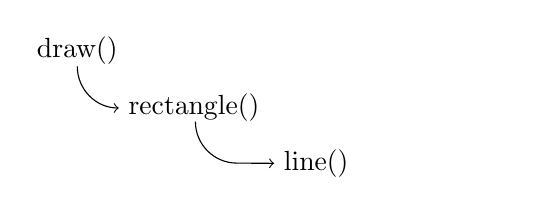
\begin{tikzpicture}
  \draw [black] (0, 0.2) node {draw()};
  \draw [black, ->] (0, 0) arc(180:270:15pt) node[anchor=west] {rectangle()};
  \draw [black, ->] (1.5, -0.7) arc(180:270:15pt) 
                    -- (2.5, -1.23) node[anchor=west] {line()};
  \draw [white] (4.6, -1.23) node {Exception!};
  \draw [white, ->] (4.5, -1.0) arc(0:90:15pt) -- (2.8, -0.47);
  \draw [white, ->] (2.6, -0.3) arc(0:90:15pt) -- (0.8, 0.225);
  \end{tikzpicture}
}

\only<4>
{
  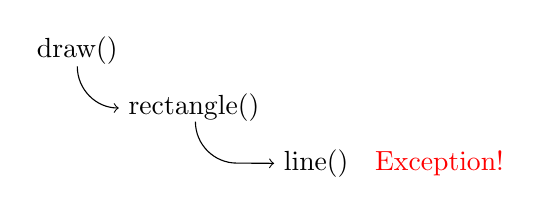
\begin{tikzpicture}
  \draw [black] (0, 0.2) node {draw()};
  \draw [black, ->] (0, 0) arc(180:270:15pt) node[anchor=west] {rectangle()};
  \draw [black, ->] (1.5, -0.7) arc(180:270:15pt) 
                    -- (2.5, -1.23) node[anchor=west] {line()};
  \draw [red] (4.6, -1.23) node {Exception!};
  \draw [white, ->] (4.5, -1.0) arc(0:90:15pt) -- (2.8, -0.47);
  \draw [white, ->] (2.6, -0.3) arc(0:90:15pt) -- (0.8, 0.225);
  \end{tikzpicture}
}

\only<5>
{
  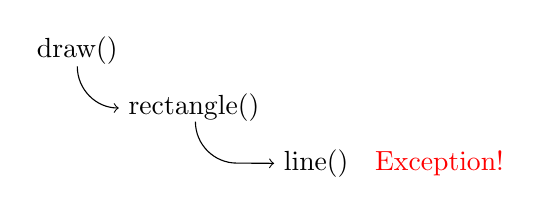
\begin{tikzpicture}
  \draw [black] (0, 0.2) node {draw()};
  \draw [black, ->] (0, 0) arc(180:270:15pt) node[anchor=west] {rectangle()};
  \draw [black, ->] (1.5, -0.7) arc(180:270:15pt) 
                    -- (2.5, -1.23) node[anchor=west] {line()};
  \draw [red] (4.6, -1.23) node {Exception!};
  \draw [white, ->] (4.5, -1.0) arc(0:90:15pt) -- (2.8, -0.47);
  \draw [white, ->] (2.6, -0.3) arc(0:90:15pt) -- (0.8, 0.225);
  \end{tikzpicture}
}

\only<6>
{
  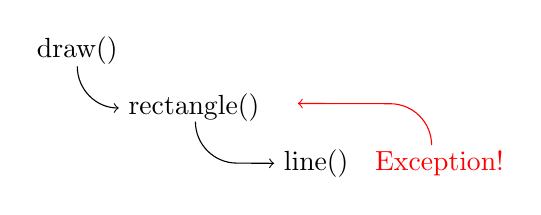
\begin{tikzpicture}
  \draw [black] (0, 0.2) node {draw()};
  \draw [black, ->] (0, 0) arc(180:270:15pt) node[anchor=west] {rectangle()};
  \draw [black, ->] (1.5, -0.7) arc(180:270:15pt) 
                    -- (2.5, -1.23) node[anchor=west] {line()};
  \draw [red] (4.6, -1.23) node {Exception!};
  \draw [red, ->] (4.5, -1.0) arc(0:90:15pt) -- (2.8, -0.47);
  \draw [white, ->] (2.6, -0.3) arc(0:90:15pt) -- (0.8, 0.225);
  \end{tikzpicture}
}

\only<7>
{
  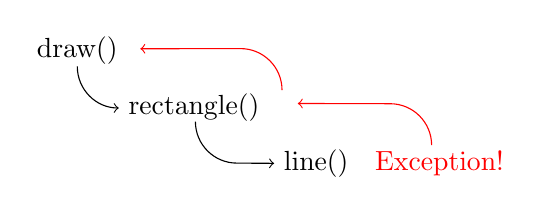
\begin{tikzpicture}
  \draw [black] (0, 0.2) node {draw()};
  \draw [black, ->] (0, 0) arc(180:270:15pt) node[anchor=west] {rectangle()};
  \draw [black, ->] (1.5, -0.7) arc(180:270:15pt) 
                    -- (2.5, -1.23) node[anchor=west] {line()};
  \draw [red] (4.6, -1.23) node {Exception!};
  \draw [red, ->] (4.5, -1.0) arc(0:90:15pt) -- (2.8, -0.47);
  \draw [red, ->] (2.6, -0.3) arc(0:90:15pt) -- (0.8, 0.225);
  \end{tikzpicture}
}
\end{figure}
\begin{itemize}
\item<1-> Funktion ruft Unterfunktionen auf.
\item<4-> Unterfunktion wirft Ausnahme.
\item<5-> Wird Ausnahme behandelt?
\item<6-> Nein: Gib Ausnahme an aufrufende Funktion weiter.
\end{itemize}
\end{frame}

\begin{frame}[fragile]{Ausnahmen ausl"osen}
Ausnahmen weiterreichen:
\begin{lstlisting}[style=Python]
try:
    f = open("spam")
except IOError:
    print "Problem while opening file!"
    raise
\end{lstlisting}
\vspace{3mm}
Ausnahmen ausl"osen:
\begin{lstlisting}[style=Python]
def gauss_solver(matrix):
    # Important code
    raise ValueError("Singular matrix")
\end{lstlisting}
\end{frame}


\begin{frame}[fragile]{Ausnahmen vs. if-Abfragen von Werten}
\onslide<1->
Ausnahmen bevorzugen!

\begin{lstlisting}
def square(x):
    if type(x) == int or type(x) == float:
        return x ** 2
    else:
        return None
\end{lstlisting}
Schlecht!

\onslide<2->
\begin{itemize}
  \item Was ist mit anderen numerischen Datentypen (komplexe Zahlen, eigene Typen)? Besser: Versuchen zu potenzieren und eventuelle Ausnahmen abfangen! $\rightarrow$ \alert{Duck-Typing}

  \item Aufrufer der Funktion kann vergessen, den R"uckgabewert zu pr"ufen (und weiterzureichen). Besser: Ausnahme ausl"osen!
\end{itemize}
\end{frame}


\begin{frame}[fragile]{Das \texttt{with}-Statement}
Einige Objekte bieten Kontext-Management an. Damit k"onnen \lstinline{try ... finally}\,-Bl"ocke einfacher geschrieben werden:
\begin{lstlisting}
with open("test.txt") as f:
    for line in f:
        print line
\end{lstlisting}
Nach dem \lstinline{with}-Block ist das Dateiobjekt stets wieder geschlossen, auch wenn im Block eine Exception auftrat.\vspace{5mm}

In Python 2.5 ist folgender Import n"otig:
\begin{lstlisting}
from __future__ import with_statement
\end{lstlisting}
\end{frame}
